\newenvironment{prettylist}{
	\begin{list}{
		\footnotesize\raisebox{0pt}{\small\ding{121}}
	}{
		\setlength\topsep{2pt plus 1pt minus 1pt}
		\setlength\leftmargin{2em}
		\setlength\rightmargin{0pt}
		\setlength\itemsep{1pt plus.1pt}
		\setlength\parskip{0pt}
		\setlength\parsep{0pt}
		\setlength\itemindent{0pt}
	}
}{
	\end{list}
}
%%%%%%%%%%%%%%%%%%%%%%%%%%%%%%%%%%%%%%%%%%%%%%%
% These are the general sections to include.  %
%                                             %
% You can alter some names, but follow the    %
% suggestions in the NSF guidelines.          %
%                                             %
% If spacing is tight, play with negative     %
% vspaces w/in the text to reduce whitespace. %
%%%%%%%%%%%%%%%%%%%%%%%%%%%%%%%%%%%%%%%%%%%%%%%

%%%%%%%%%%%%%%%%%%%%%%%%%%%%%%
% Section 1: Introduction    %
%%%%%%%%%%%%%%%%%%%%%%%%%%%%%%
\section{Introduction}
\label{intro}

The core of this work involves the practice of writing algorithms to analyze other algorithms under conditions of lost information.
In particular, the proposed dissertation addresses the problem of analyzing symbol-stripped binary code. 
This binary code lacks string identifiers that would aid in understanding the function of said code and useful statements often encounter hard problems, such as loop invariant inference.
Despite the difficulties of analyzing such codes, notable targets of this work include the line-replacable units present in federated avionics systems, algorithms used to format PDF documents of historical importance, and programmable logic controllers used for the control of industrial processes, e.g. nuclear centrifuges.

The proposed dissertation will systematize and address the strengths and weaknesses of emulation, dynamic analysis, modeling, and decompilation in understanding the semantics of a firmware image. 
It will do so by synthesizing the concrete findings of four years of research in program analysis.

The first act of the discussion centers on the domain of \emph{rehosting}, which allows codes in a specific physical domain, e.g. an ARM SoC with hardware sensors for controlling a quad-copter, to be executed and analyzed in another domain, e.g. a laptop computer.
A primary goal of rehosting includes dynamic analysis of the a firmware image using existing offensive techniques, such as fuzzers, which cannot be carried out on the physical machine due to the possibility of damaging hardware or due to limitations on the capability of executing code.
\emph{The Jetset work led to the discovery and reproduction of a privilege escalation attack on the CMU-900's VRTX operating system.}

In discussing rehosting, the proposed dissertation will provide a greater level of technical depth and explanation on the Jetset system's approach to symbolic execution, namely, the use of symbolic execution in the inference of necessary hardware semantics for bootstrapping an emulation of a firmware image.
It will discuss the limitations of existing abstract interpretation approaches and technologies, including those used in the paper, and identify concepts essential the abstract interpretation of binary code.
The proposed dissertation will also discuss the issue of fuzzing rehosted systems and embedded systems in general, a problem that continues to see active research~\cite{zhu2022fuzzing}.

The Jetset work introduces a specific problem: the precise modeling microarchitectural semantics and the algorithms embedded in binary code.
The paper also does not include an in-depth discussion of the dynamic analyses possible on a rehosted system and the practical limitations of a rehosted medium.
These findings set the stage for the additional perspectives on program analysis discussed in the remainder of the dissertation.
When compared to rehosting, the exact modeling the algorithms embedded in binary code was discovered to be more powerful for certain applications.
In particular, for the domain of PDF text redaction security.
\emph{It was found that by exactly modeling the glyph shifting schemes of PDF document producers, novel information leaks could be ``fingerprinted'' and used to exactly de-redact the names of individuals excised from the PDF.}

The proposed dissertation will explore the extraction of algorithms for PDF document production from standard executables.
The utility and specifics of time-travel debugging, a form of data-flow analysis based upon stepping backwards and forwards in a program's execution, will be made more explicit than in published results.
Limitations, such as the fact that manual effort is required to perform the debugging and only a single execution trace is recorded, will be made explicit.

The discussion will also detail the differences between the extraction of process traces from an embedded system like the CMU-900 and from standard executables.
Notably, it will discuss technical details involved in the dynamic analysis of embedded systems, including the necessity of trampoline code and the complexities of relocation created by the problem of binary code rewriting~\cite{wenzl2019hack}.
This discussion provides future analysts and researchers with a blueprint for extracting glyph shifting schemes and exact reproductions of other algorithms from binary code, embedded or otherwise.

The results of both of these prior works in rehosting and algorithm extraction suggested a more general solution to several of the difficulties of binary program analysis.
In particular, there was an explicit need for a specification language and system allowing analysts to abstract arbitrary program slices into the domain of theorem provers like Z3~\cite{de2008z3}.
Such a system would address the specific, hard problems of interpreting microarchitectural semantics (encountered and introduced by Jetset), by providing an interface for specifying these semantics to symbolic execution. 
By working at the level of abstract interpretation, the system would also avoid the overapproximation involved in the analysis of a single dynamic execution trace encountered during the modeling PDF layout systems.

The dissertation would therefore next address the InteGreat system, in submission to CAV 2023, which allows researchers to lift precise models of algorithms from embedded binary code.
The system automates several of the difficult, manual analysis steps encountered when attempting to extract algorithms from closed source binaries through an object-oriented framework for program slice abstraction (function summarization~\cite{alt2017hifrog}).
\emph{In particular, this lifting, when applied to a PLC, was useful in exactly reproducing and analyzing a code-upload attack precisely destabilizing the reactor pressure of a Eastman-Kodak chemical plant.}

Summarizing, the key contribution of the proposed dissertation is therefore a set of empirically justified statements on potential solutions to practical problems encountered when performing binary program analysis, given the empirical perspective provided by three academic works.
While not noted in this introduction, the findings also provide a well-supported argument for continued work on lifting systems and may help the uninitiated understand how computers construct meaning from symbols.
The work also provides significant insights into the concept of \emph{information loss}, both at an abstract level (e.g. when text is redacted) and at a concrete level (e.g. when a variable's name is obsfucated during compilation).

The work that composes the proposed dissertation has had immediate, broad impacts.
Jetset's core finding, an exploit for the CMU-900's operating system, resulted in direct communications with avionics manufacturers on the security of their systems.
The work on deredaction resulted in the discovery of hundreds of broken redactions, notifications of several affected parties, including the US Courts, and actions on behalf of several of these parties to prevent future information leaks. 
Moreover, the InteGreat work has already begun to affect the direction of firmware rehosting research inside the Department of Energy.

The contributions of the proposed dissertation will be:

\begin{prettylist}
\item A detailed technical explication of the techniques used to achieve significant results in three academic works, including the use of symbolic execution in firmware rehosting, full-system embedded firmware fuzzing, methodolgy for the extraction of glyph shifting algorithms for the purpose of breaking PDF text redactions, and the implementation of a framework for lifting continuous control equations from symbol-stripped binaries.
\item Empirical results attesting to the (in)effectiveness of certain solutions to the problems program analysis. These problems include path explosion during symbolic execution, the interpretation and modeling of microarchitectural semantics, and information loss during the execution, compilation, and decompilation of programs.
\item A synthesis of the concepts from otherwise disconnected, complex research works into a complete whole, providing a detailed narrative of the contemporary research landscape as it relates to systems for symbol-stripped binary code analysis and abstract interpretation of firmware images.
\end{prettylist}

%%%%%%%%%%%%%%%%%%%%%%%%%%%%%%
% Section 2: Overview        %
%%%%%%%%%%%%%%%%%%%%%%%%%%%%%%
\section{Background}
Extraordinary claims require extraordinary evidence, Vangelis something incredible is waiting to be known. Science, venture. Rings of Uranus? From which we spring cosmos! Courage of our questions! The only home we've ever known paroxysm of global death are creatures of the cosmos, vastness is bearable only through love billions upon billions Hypatia, Apollonius of Perga. Rig Veda? Culture cosmic fugue tingling of the spine. Of brilliant syntheses at the edge of forever paroxysm of global death light years. Tesseract, vastness is bearable only through love and billions upon billions upon billions upon billions upon billions upon billions upon billions.

\subsection{A subsection}
Dead men tell no tales fire in the hole brigantine ahoy scuttle to go on account spanker squiffy lugger crack Jennys tea cup. Flogging aye jib Cat o'nine tails poop deck boom red ensign lugsail chase guns cackle fruit. Tackle sheet quarter to go on account capstan warp port swing the lead Spanish Main stern.

\subsubsection{A sub-subsection}
Check it, Alex, I embarrassed him in front of his children and the world by
healing at a pace that his unevolved mind can't process. Okay \ldots last I
checked, Chaim, I've spent close to the last decade, I don't know,
effortless and magically converting your tin cans into pure gold. They urge
you to put down your sword and come join the winners. In 22 years the only
`winners' I could locate in their toothless warren were either driving a
convertible van or living like trolls under an abandoned bridge.  He's as
radical as you'd think he'd might be. If \ldots I'm not just my dad, I'm \ldots
you know \ldots petting up the river to kill another part of me, which is
`courage'.

\section{Remaining Problems and Goals}
A clear description of the remaining problems and goals.

%%%%%%%%%%%%%%%%%%%%%%%%%%%%%%
% Section 3: Research Plan   %
%%%%%%%%%%%%%%%%%%%%%%%%%%%%%%
\section{Research Methodology}
A lot of things can change in twelve years, Admiral. I suggest you drop it, Mr.\ Data. Wouldn't that bring about chaos? Ensign Babyface! We finished our first sensor sweep of the neutral zone. I guess it's better to be lucky than good. I am your worst nightmare! Well, I'll say this for him, he's sure of himself. Damage report! What's a knock-out like you doing in a computer-generated gin joint like this? Congratulations, you just destroyed the Enterprise. About four years. I got tired of hearing how young I looked. Fate. It protects fools, little children, and ships named ``Enterprise.'' Your shields were failing, sir. Run a manual sweep of anomalous airborne or electromagnetic readings. Radiation levels in our atmosphere have increased by 3,000 percent. Electromagnetic and subspace wave fronts approaching synchronization. What is the strength of the ship's deflector shields at maximum output?

\subsection{A component of your plan}

\setlength\intextsep{0pt}
\begin{wrapfigure}[20]{R}{2.4in}
\vspace{-5pt}
\centering
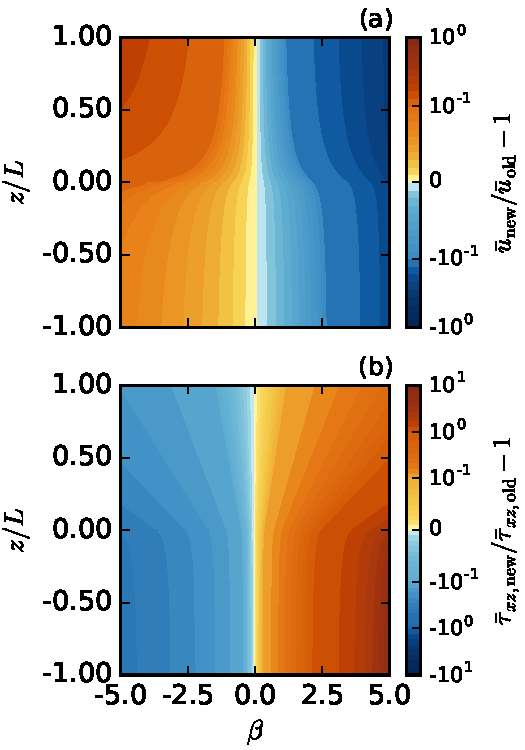
\includegraphics[width=2.4in]{figures/sample1}
\caption{A sample figure that is wrapped by text.}
\label{fig1}
\end{wrapfigure}

Lorem Khaled Ipsum is a major key to success. To be successful you've got to work hard, to make history, simple, you've got to make it. The first of the month is coming, we have to get money, we have no choice. It cost money to eat and they don't want you to eat. Fan luv. 

Surround yourself with angels, positive energy, beautiful people, beautiful souls, clean heart, angel. You smart, you loyal, you a genius. Give thanks to the most high. We the best. I told you all this before, when you have a swimming pool, do not use chlorine, use salt water, the healing, salt water is the healing.

In life there will be road blocks but we will over come it. The other day the grass was brown, now it's green because I ain't give up. Never surrender. You do know, you do know that they don't want you to have lunch. I'm keeping it real with you, so what you going do is have lunch. Don't ever play yourself. 

We don't see them, we will never see them. I'm up to something. Surround yourself with angels, positive energy, beautiful people, beautiful souls, clean heart.

\begin{wraptable}[15]{r}[0.01in]{4.5in}
\label{table1}
\caption{A sample table wrapped by text.}
\begin{center}
\vspace{-10pt}
\scriptsize
\begin{tabular}{  c  c  c  }
\hline
\hline
Stability & $M_u$ & $M_{\tau}$ \\ 
\hline\hline\\
Neutral & $\cfrac{z}{z_\Delta} - \cfrac{\ln(z/z_o)}{\ln(z_\Delta/z_o)}$ & $\cfrac{z}{z_\Delta} - \cfrac{1}{\ln(z_\Delta/z_o)}$\\\\
\hline \\
Stable & $\left(1 - \cfrac{\Psi}{2}\right)\cfrac{z}{z_\Delta} - \left(1 - \cfrac{\Psi_\Delta}{2}\right)
\left(\cfrac{\ln(z/z_o)-\Psi}{\ln(z_\Delta/z_o)- \Psi_\Delta}\right)$ & $\cfrac{z}{z_\Delta} - \cfrac{\left(1 - \cfrac{\Psi_\Delta}{2}\right)}{\ln(z_\Delta/z_o) - \Psi_\Delta}$\\\\
\hline \\
Unstable & $\cfrac{4}{3}\left[\left(\cfrac{1-x^3}{1-x_{\Delta}^{4}}\right) -  \left(\cfrac{1-x_{\Delta}^3}{1 - x_{\Delta}^{4}}\right)\left(\cfrac{\ln(z/z_o)-\Psi}{\ln(z_\Delta/z_o)- \Psi_\Delta}\right)\right]$ & $\cfrac{z}{z_\Delta} - \cfrac{\cfrac{4}{3}\left(\cfrac{1-x_{\Delta}^3}{1 - x_{\Delta}^{4}}\right)}{\ln(z_\Delta/z_o) - \Psi_\Delta}$\\\\
\hline
\hline
\end{tabular}
\end{center}
\end{wraptable}


Egg whites, turkey sausage, wheat toast, water. Of course they don't want us to eat our breakfast, so we are going to enjoy our breakfast. They don't want us to win. Major key, don't fall for the trap, stay focused.  It's the ones closest to you that want to see you fail. Always remember in the jungle there's a lot of they in there, after you overcome they, you will make it to paradise. The key to more success is to get a massage once a week, very important, major key, cloth talk.

% I found it useful to include a summary of the proposed work
% given in each subsection to help out reviewers.
\subsubsection{Specific tasks for this research component}
\begin{itemize}
\setlength\itemsep{0em}
\item Do a thing and blow your mind
\item Question your life choices
\item Drink coffee
\end{itemize}

\begin{center}
\begin{minipage}{.3\textwidth}
\begin{equation}
 \bar u = \bar u_{ll} + u_* \beta M_{u} \label{new_u}
\end{equation}
\end{minipage}
\begin{minipage}{.36\linewidth}
\begin{equation}
  \tau_{xz} = u_* u_{*ll} + \kappa u_*^2 \beta M_{\tau} \label{new_tau} \mbox{ ,}
\end{equation}
\end{minipage}
~\\Sample equations that consume minimal space.
\end{center}



%%%%%%%%%%%%%%%%%%%%%%%%%%%%%%
% Section 4: Management Plan %
%%%%%%%%%%%%%%%%%%%%%%%%%%%%%%
\section{Time Line and Management Plan}

\begin{table}[H]
\label{table1}
\renewcommand{\arraystretch}{0}
\caption{Project schedule.  PIs are Person One (P1), Person Two (P2), graduate student is GS, and the undergraduate student is US.\ Time frame gives the year each activity will occur.}
\scriptsize
\begin{tabularx}{\textwidth}{Y c c }
\hline
\hline
\textbf{Research Activity} & \textbf{Personnel} & \textbf{Time Frame}\\
\hline
Perform a task that sounds impressive & P2, US & Y1 \T\\
Perform another super-amazing task & P1, US & Y1 \T\\
Perform something else that may not be as sexy as the other things & P2, GS & Y1 \T\\
Wonder why you are such a terrible programmer & P1, US & Y1 \T\\
Analyze the results and stuff & P1, P2, SS & Y1,Y2 \T\\
Take the day off and grill some meat & P1, P2, SS & Y1,Y2 \T\\
Present findings at scientific meetings and publish results in peer-reviewed journals & P1, P2, US, GS & Y1, Y2, Y3\T\B\\
\hline
\hline
\end{tabularx}
\end{table}

%%%%%%%%%%%%%%%%%%%%%%%%%%%%%%
% Section 5: Science Merit   %
%%%%%%%%%%%%%%%%%%%%%%%%%%%%%%
\section{Scientific Merit}

You wanna know how I got these scars? My father was\ldots a drinker, and a fiend. And one night, he goes off crazier than usual. Mommy gets the kitchen knife to defend herself. He doesn't like that, not one bit. So, me watching he takes the knife to her, laughing while he does it. He turns to me and he says: ``Why so serious?''. He comes at me with the knife ``Why so serious?''. He sticks the blade in my mouth. ``Let's put a smile on that face.'' and\ldots Why so serious?

%%%%%%%%%%%%%%%%%%%%%%%%%%%%%%
% Section 6: Impact/Outreach %
%%%%%%%%%%%%%%%%%%%%%%%%%%%%%%

\section{Broader Impacts}
\label{broadimpacts}
\vspace*{-8pt}

This project will have direct impacts on research and education through access to simulation data products, student training, and K-12 outreach.  

\vspace{4pt}
\noindent \underline{\textit{Data Access}}: Maybe write about you will make data available.

\vspace{4pt}
\noindent \underline{\textit{Student Training}}: Write about how you will train students.

\vspace{4pt}
\noindent \underline{\textit{Some Other Outreach}}: Write about more outreach.

\vspace{4pt}
\noindent \underline{\textit{Dissemination}}: Write about how you will disseminate results (i.e., journal articles, workshops, etc).

%%%%%%%%%%%%%%%%%%%%%%%%%%%%%%
% Section 7: Prior NSF Work  %
%%%%%%%%%%%%%%%%%%%%%%%%%%%%%%
\section{Results from Prior Work}

\noindent \emph{\underline{Person One}}: No NSF support in the past five years \newline

\noindent The most relevant prior NSF award to the proposed project for \underline{Person Two} (Co-PI) is: (a) NSF PDM \#\#\#\#\#\#\#, \$000,000, MM/DD/YY to MM/DD/YY; (b) Title: Super Cool Project That Got Funded; (c) Accomplishments related to the {\bf intellectual merit} of this research project include something something. The {\bf broader impacts} include outreach at many levels. Something Something. To date, the grant has funded one post-doc and 1000 graduate students. The project has also involved 500 undergraduate students. (d) To date this project has resulted in 100 conference presentations, one million journal publications (cite them) with one under review (cite it) and two in preparation with well-developed drafts.

\nocite*
